\section{Architecture}
\label{arch} 
We propose a distributed collaborative scheme that existing domain mail servers can use along with other techniques (conventional blacklists and content-based filtering schemes), for detecting spam. Figure~\ref{fig:architecture} provides a high level overview of the architecture along with the overlay network topology that is used for sharing information. The architecture diagram shows a logical separation between super-nodes that are connected in a peer-to-peer fashion to aggregate information for clustering. The super-nodes form the backend of the system. We can have settings where domain mail servers or nodes at an enterprise having relationship with the domains, can act as super nodes. The peer-to-peer network of super-nodes forms the backend of our system. These nodes aggregate the information about the traffic of spammers and perform clustering. The cluster information is sent back to the domain mail servers. Classification of new received emails is performed locally at the domain mail servers.

Currently we have implemented the backend of the system that has a set of super-nodes running the clustering algorithm in a distributed fashion. In section~\ref{future} we discuss further work that will make the system scalable and deployable in the real-world. Section~\ref{arch-cluster} explains the backend architecture and gives details on how clustering is performed in the system. In section~\ref{arch-classify} we explain how the domain mail servers can use the cluster information to detect spammers. The distributed implementation of the backend is discussed in section~\ref{sec:distP2}.

\begin{figure}[t]%{4.25in}
\centering
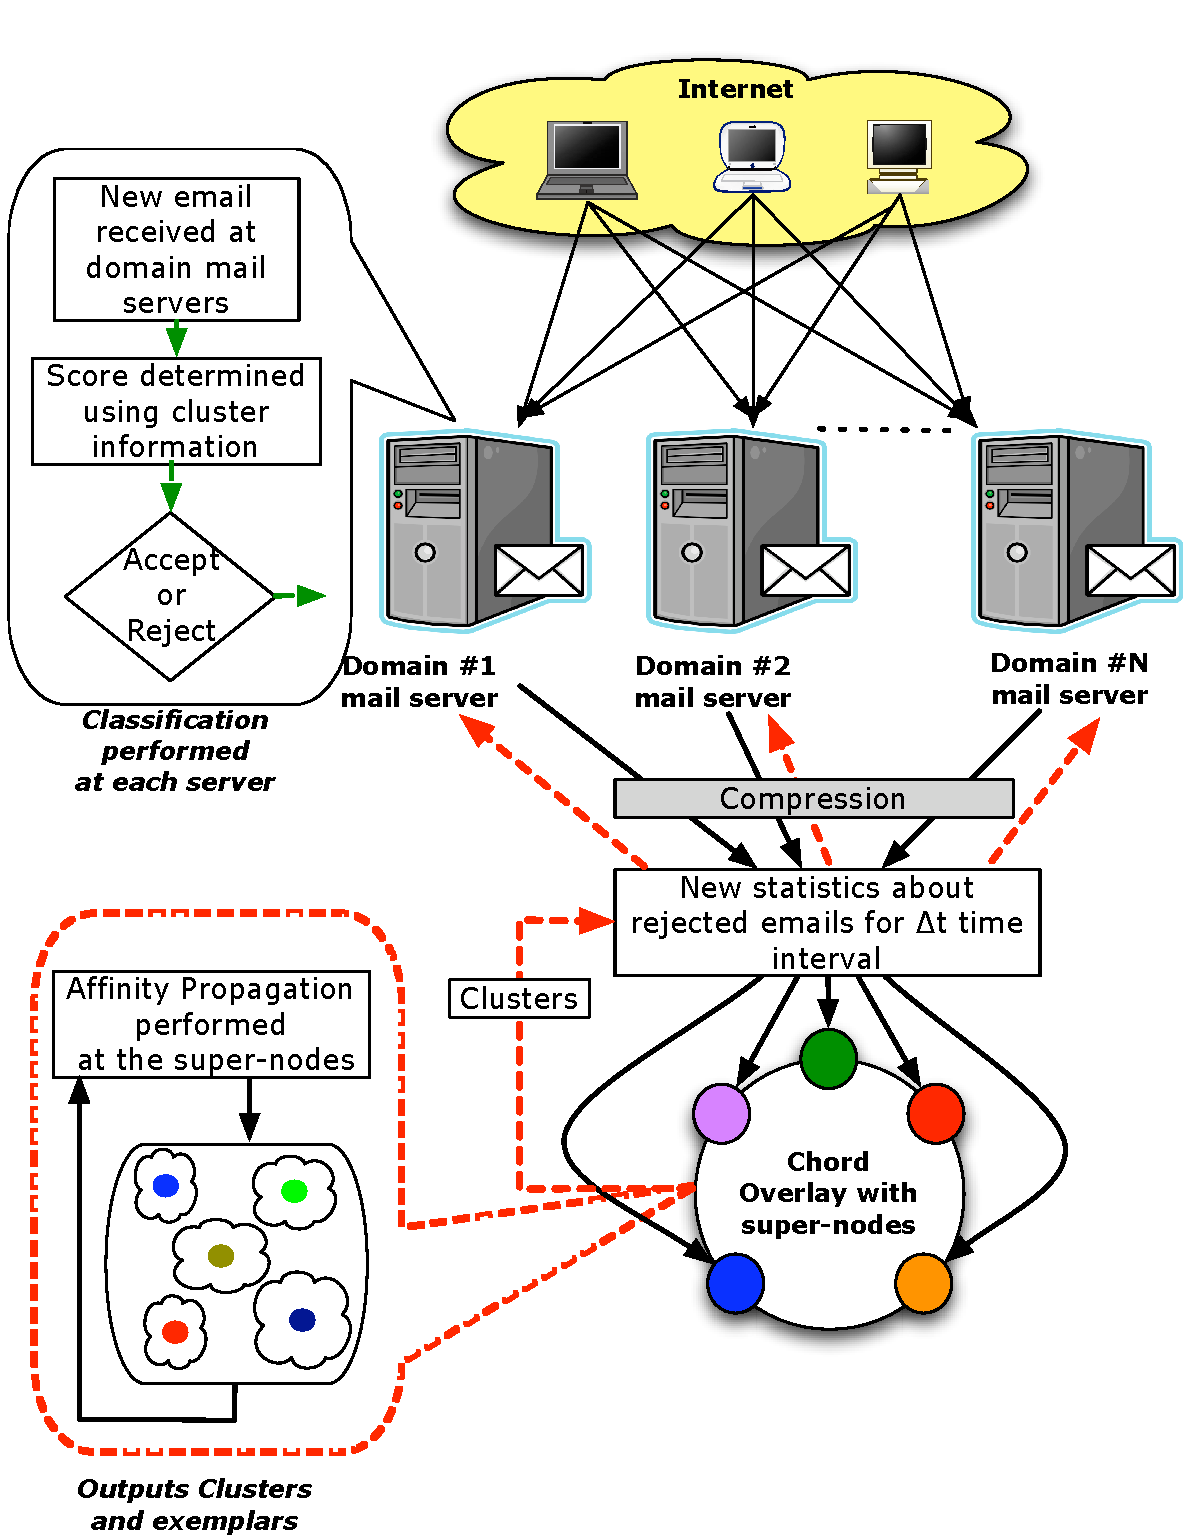
\includegraphics[width=0.45\textwidth]{figures/architecture.pdf}
\caption{High level overview of the architecture. The compression block is not implemented currently}
\label{fig:architecture}
\end{figure}
\subsection{Clustering}
\label{arch-cluster}

Affinity propagation calculates clusters that are refined iteratively by performing clustering over the information periodically collected from domain mail servers. This information for clustering includes details regarding the frequency of emails a domain rejects from spammers. This can be obtained from domain mail servers that use conventional filters to filter spam~\cite{spamassassin} . The list can also be enriched from user feedback on spam emails as well. We use the dataset that \emph{SpamTracker} \cite{bb} used for clustering, which contains the information regarding the frequency of emails from spammers that a domain receives. The dataset is from an email hosting provider's decisions about early mail rejects from hundreds of domains. More details about the data can be found in section~\ref{sec:data}. 

The spammer's activity at a particular domain is sent to a super-node that is geographically close to the domain mail server. Chord is used to lookup the super-node that corresponds to the location where the data of the IP address is aggregated. The super-nodes aggregate the IP address activity across all domains. The aggregated information for each IP address represents the row in matrix $M$ (Equation~\ref{eq:collapse}) for the IP address.  Section~\ref{future} discusses details on how aggregation can be accomplished with domain mail servers acting as super-nodes connected in a peer-to-peer network in a scalable fashion. 

After the aggregation has been performed, similarity of an IP address's sending pattern with other IP address is calculated (Equation~\ref{eq:similarity}). This similarity information forms the basis for clustering. The clusters, calculated by running affinity propagation, are sent back to the domain mail servers, communicating the sending patterns of spammers.

The clusters are refined periodically after \emph{$\bigtriangleup t$} time interval. We choose \emph{$\bigtriangleup t$} to be 6 hours (the same value as chosen by Ramachandran \cite{bb}) but this can be made configurable and changed randomly to overcome evasion \footnote{Refer to Section~\ref{future} for further discussion on evasion}. Email rejection information for \emph{$t+\bigtriangleup t$} is collected and sent to the super-nodes for updating the clusters.
\subsection{Classification}
\label{arch-classify}

Whenever a domain mail server receives an email it creates or appends the sending information for the IP address to its own logs. This information is shared with other mail servers after a brief period of time. The server then calculates the score of the IP address' sending pattern with respect to the recent cluster information stored locally. Classification can be performed in real-time and locally. The magnitude of the score \emph{S} computed using Equation~\ref{eq:score} determines how closely the sending pattern of the IP address matches a spammer's sending pattern. Each domain mail server can incorporate its own threshold value for the score and decide actions to be performed against emails that have a higher score than the threshold.

\subsection{P2 Distributed Implementation}
\label{sec:distP2}

Our current work involves implementation of the backend of the system. The backend has a set of super-nodes running the affinity propagation clustering algorithm in a distributed fashion. Affinity propagation is implemented in P2 and is run on all super-nodes. The affinity propagation overlog has three main relations similarity, responsibility and availability. The similarity relation stores the similarity each local IP address has with other IP addresses. Responsibilities and availabilities are initialized to zero and updated at regular time intervals equal to AP\_EPOCH. Relation sentResponsibility is used to store the responsibilities sent by a node. This information saves us from doing a round-trip while calculating the exemplars. Refer to Appendix~\ref{appendix} to have a look at the detailed overlog. For brevity, we have not shown the damping factor calculations, initialization messages and Chord integration for lookup of data location. Materialized table variable stores the location of the IP address. We have modified the algorithm to work for multiple variables per node and the localVariable table stores the information of IP addresses associated with a super-node.

Each super-node stores information regarding the similarity of a set of IP addresses. The similarity is calculated using Equation~\ref{eq:similarity}. 
These super-nodes send messages, locally or to remote nodes that have IP addresses with similar sending behavior to the local IP addresses.

To reduce the amount of information aggregated at the super-nodes, we took a greedy approach for performing \emph{cluster compression}. This approach reduces the number of IP addresses that have to be clustered and thus reduces the computation performed for clustering. Each row in the complete matrix $M$ (Equation~\ref{eq:collapse}) is classified with the cluster averages. Rows having high scores (Equation~\ref{eq:score}) are removed from the matrix and their sending information is incorporated into the previous clusters. This is computed by averaging the new rows and the cluster (Equation~\ref{eq:cavg}) to get the updated clusters. A new matrix is formed, which includes the new clusters along with a mutually exclusive random sample of IP addresses that sent email during this same \emph{$\bigtriangleup t$} interval. This \emph{n}x\emph{d} matrix is used for affinity propagation as before. 